\usetikzlibrary{arrows.meta}
\begin{enumerate}
\item \textbf{นิยามลิมิต และการหาลิมิตจากกราฟ}

\begin{minipage}{0.55\textwidth}
\begin{itemize}
\item $\limx{a^-} f(x)$ อ่านว่า  \hrulefill
\item $\limx{a^+} f(x)$ อ่านว่า  \hrulefill
\item $\limx{a} f(x)$ อ่านว่า \hrulefill

จะหาค่าได้ก็ต่อเมื่อ \hrulefill

\end{itemize}
จงหาลิมิตต่อไปนี้ เมื่อกำหนดกราฟของ $f(x)$ ให้ด้านขวา
\begin{tasks}[after-item-skip = 30pt, after-skip = 30pt](3)
\task $\limx{-1^-} f(x)$
\task $\limx{-1^+} f(x)$
\task $\limx{-1} f(x)$
\task $\limx{0^-} f(x)$
\task $\limx{0^+} f(x)$
\task $\limx{0} f(x)$
\task $\limx{2^-} f(x)$
\task $\limx{2^+} f(x)$
\task $\limx{2} f(x)$
\end{tasks}
\medskip
\end{minipage}
\begin{minipage}{0.4\textwidth}
\centering
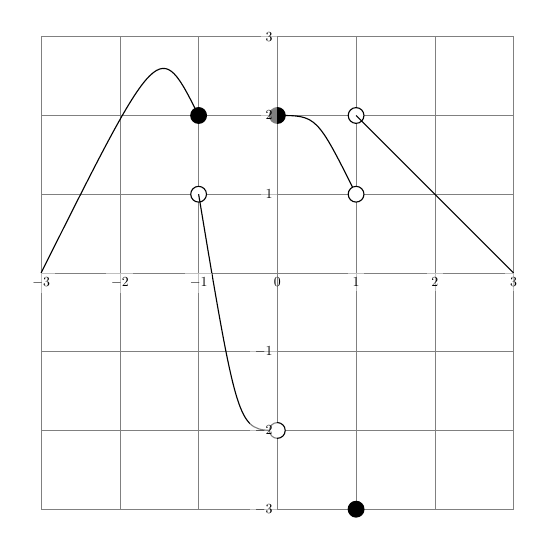
\begin{tikzpicture}
\axes{-3.2}{3.2}{-3.2}{3.2};
\draw[very thin, gray] (-3,-3) grid (3,3);
\draw (-3,0) .. controls (-1.5,3) .. (-1,2);
\filldraw[fill = black] (-1, 2) circle [radius = 0.1cm];
\filldraw[fill = white] (-1, 1) circle [radius = 0.1cm];
\draw (-1,1) .. controls (-0.5,-2) .. (0,-2);
\filldraw[fill = white] (0, -2) circle [radius = 0.1cm];
\filldraw[fill = black] (0, 2) circle [radius = 0.1cm];
\draw (0,2) .. controls (0.5,2) .. (1,1);
\filldraw[fill = white] (1, 1) circle [radius = 0.1cm];
\filldraw[fill = black] (1, -3) circle [radius = 0.1cm];
\filldraw[fill = white] (1, 2) circle [radius = 0.1cm];
\draw (1,2) -- (3,0);
\foreach \x in {-3,-2,-1,1,2,3}
{
	\node at (\x,0) [below, scale = 0.5, fill = white, fill opacity = 0.5, text opacity = 1] {$\x$};
	\node at (0,\x) [left, scale = 0.5, fill = white, fill opacity = 0.5, text opacity = 1] {$\x$};
}
\node at (0,0) [below, scale = 0.5, fill opacity = 0.5, text opacity = 1] {$0$};
\end{tikzpicture}
\captionof{figure}{กราฟ $y = f(x)$ สำหรับโจทย์ข้อที่ \theenumi}
\label{fig:limit_graph_ex2}
\end{minipage}

\item \textbf{การหาลิมิตโดยการวิเคราะห์ฟังก์ชัน}

จงคำนวณค่าของฟังก์ชันลงไปในตารางต่อไปนี้ พร้อมประมาณค่าลิมิตของฟังก์ชัน

\begin{tasks}[after-item-skip = 20pt, after-skip=20pt](1)
\task $\limx{1} \frac{x^3-1}{x-1}$

\medskip

\begin{tblr}{colspec={|c|X[c]|X[c]|X[c]|X[c]|X[c]|X[c]|}, rowspec={|Q[10pt]|Q[30pt]|}, cells={mode=math}}
x &  0.9 &  0.99 &  0.999 &  1.001 &  1.01 &  1.1 \\
f(x) =  \frac{x^3-1}{x-1}  &&&&&& \\
\end{tblr}

\medskip
ฉะนั้น เราจึงสรุปได้ว่า \blank[2]

\task $\limx{0} \frac{\sin(x)}{x}$ \mathnote{ในทางคณิตศาสตร์ การคำนวณ $\sin(x)$ จะใช้มุม $x$ ที่มีหน่วยเป็น \blank}

\medskip

\begin{tblr}{colspec={|c|X[c]|X[c]|X[c]|X[c]|X[c]|X[c]|}, rowspec={|Q[10pt]|Q[30pt]|}, cells={mode=math}}
x &  -0.1 &  -0.01 &  -0.001 &  0.001 &  0.01 &  0.1 \\
f(x) =  \frac{\sin(x)}{x}  &&&&&& \\
\end{tblr}

\medskip
ฉะนั้น เราจึงสรุปได้ว่า \blank[2]

\end{tasks}

\newpage
% พีชคณิตของลิมิต
\item \textbf{พีชคณิตของลิมิต} 

กำหนด $a,c$ เป็นค่าคงตัวแล้ว
\[ \limx{a} c = \blank, \qquad \limx{a} x = \blank \]

จงหาค่าของลิมิตต่อไปนี้ โดยการเขียนเครื่องหมายลิมิตทุกขั้นตอน จนกว่าจะคำนวณลิมิต
\begin{tasks}[after-item-skip = 60pt, after-skip=60pt](3)
\task $\limx{0} 4$
\task $\limx{-1} x$
\task $\limx{3} x^2$
\task $\limx{1} (x+2)$
\task $\limx{3} (x^2+1)$
\task $\limx{1} (x+1)(x+2)(x+3)$
\end{tasks}

% ลิมิตอนันต์ และลิมิตที่มีค่าเป็นอนันต์
\item \textbf{ลิมิต ณ อนันต์ และลิมิตที่มีค่าเป็นอนันต์}

\begin{itemize}
\item ลิมิต ณ อนันต์ คือ \hrulefill
\item ลิมิตที่มีค่าเป็นอนันต์ คือ  \hrulefill
\end{itemize}

จงระบุว่าลิมิตต่อไปนี้เป็นลิมิตประเภทใด พร้อมหาค่าด้วยการวาดกราฟหรือสร้างตารางแทนค่า
\begin{tasks}[after-item-skip = 60pt, after-skip=60pt](4)
\task $\limx{0^-} \frac{1}{x^2}$
\task $\limx{0^+} \frac{1}{x^2}$
\task $\limx{\infty} \frac{1}{x^2} $
\task $\limx{-\infty} \frac{1}{x^2} $
\end{tasks}

% การหาลิมิตเมื่อฟังก์ชันอยู่ในรูป 0/0
\item \textbf{การหาลิมิตเมื่อฟังก์ชันอยู่ในรูป $\frac{0}{0}$}

กำหนด $\limx{a} \frac{f(x)}{g(x)}$ ซึ่ง \blank แล้วมีความเป็นไปดังต่อไปนี้
\begin{itemize}
\item ลิมิตหาค่าได้ โดยเราหาลิมิตได้ด้วยการ \blank
\item ลิมิตมีค่าเป็น \blank
\item \blank
\end{itemize}

จงหาค่าของลิมิตต่อไปนี้
\begin{tasks}[after-item-skip = 100pt, after-skip = 100pt](5)
\task $\limx{0} \frac{x^3+3x}{x}$
\task $\limx{0} \frac{2x^5 - 3x^4}{x^3}$
\task $\limx{2} \frac{x^2-4}{x-2}$
\task $\lim_{h \to 0} \frac{(h+1)^2-1}{h}$
\task $\limx{3} \frac{x^2-9}{x^2-4x+3}$
%\task* $\limx{0} \frac{(A+x)^2-A^2}{x}$ เมื่อ $A$ เป็นค่าคงตัว
\end{tasks}

\end{enumerate}
